\section{Matrix Multiplication}
\subsection{Problem Statement}
Implement Iterative Matrix Multiplication, Divide-and-Conquer Matrix Multiplication and Strassen's Matrix Multiplication algorithm to multiply two matrix of valid dimension. 
Compare the 3 algorithms based on various input size on randomly generated matrices.  The comparison metric should be the execution time of each matrix multiplication algorithm.
\subsection{Code}
\begin{code}
    \caption{matrix\_multiplication.cpp}
    \cppcode{../recursive_matmul.cpp}
    \label{code:matmul}
\end{code}
\subsection{Output}
\begin{figure}[H]
    \centering
    \begin{subfigure}[b]{0.4\textwidth}
        \centering
        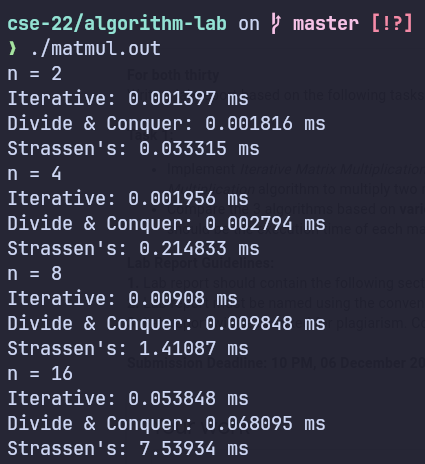
\includegraphics[width=\textwidth]{./img/lab3/matmul-1.png}
    \end{subfigure}
    \hfill
    \begin{subfigure}[b]{0.4\textwidth}
        \centering
        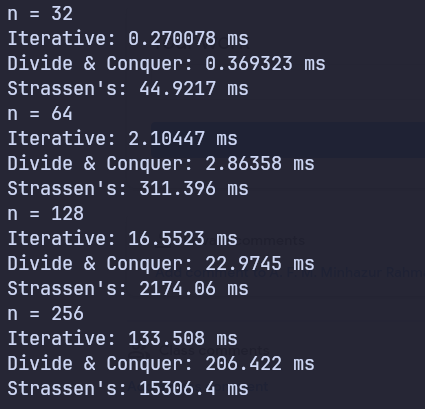
\includegraphics[width=\textwidth]{./img/lab3/matmul-2.png}
    \end{subfigure}
    \caption{Execution time for matrix multiplication}
    \label{fig:task1}
\end{figure}

\subsection{Result}

\begin{table}[H]
    \centering
    \caption{Comparison table for Iterative \& Divide \& conquer and 
    Strassen's Matrix multiplication algorithm execution time}
    \label{tab:comp}
    \begin{tabular}{lrrr}
        \toprule
        \multicolumn{1}{c}{Input Size} & \multicolumn{1}{c}{Iterative (ms)} & \multicolumn{1}{c}{Divide \& Conquer (ms)} & \multicolumn{1}{c}{Strassen's (ms)} \\
        \midrule
        $2\times2$   & 0.001397 & 0.001816 & 0.033315\\
        $4\times4$   & 0.001956  & 0.002794 & 0.214833 \\
        $8\times8$  & 0.00908  & 0.009848 & 1.41087 \\
        $16\times16$  & 0.053848 & 0.068095 & 7.53934 \\
        $32\times32$ & 0.270078 & 0.369323 & 44.9217\\
        $64\times64$ & 2.10447 & 2.86358 & 311.396 \\
        $128\times128$ & 16.5523 & 22.9745 & 2174.06  \\
        $256\times256$ & 133.508 & 206.422 & 15306.4 \\
        \bottomrule
    \end{tabular}
\end{table}

\subsection{Analysis \& Discussion}
The iterative algorithm demonstrates consistent performance 
and scales predictably with increasing input size. 
Its time complexity is $O(n^3)$, which aligns with theoretical expectations. As seen in the results, the runtime increases steadily, from 0.001397 ms for 
2×2 matrices to 133.508 ms for 
256×256 matrices. Despite its cubic complexity, the iterative approach has minimal overhead, making it an efficient choice for small to medium-sized matrices. Its straightforward implementation also contributes to its practicality in many applications.

The divide-and-conquer (recursive) algorithm shares the same 
 $O(n^3)$ time complexity but incurs additional overhead due to recursive function calls. This overhead is noticeable for smaller matrices, where it performs slightly worse than the iterative algorithm. For example, at 
2×2, the recursive approach takes 0.001816 ms, which is slower than the iterative method's 0.001397 ms. As the input size grows, the performance gap widens, with the recursive algorithm taking 206.422 ms for 
256×256 matrices, compared to the iterative method's 133.508 ms. The recursion overhead thus limits its practicality for general use.

Strassen’s algorithm theoretically offers better time complexity, approximately 
$O(n^{2.81})$, by reducing the number of multiplications required. However, in practice, it incurs significant overhead due to matrix partitioning, additional additions and subtractions, and increased recursion depth. This overhead dominates for smaller and moderately sized matrices, resulting in much slower performance compared to both iterative and recursive methods. For instance, at 
64×64, Strassen’s method takes 311.396 ms, compared to 2.10447 ms and 2.86358 ms for the iterative and recursive methods, respectively. For larger sizes, such as 
256×256, the overhead becomes even more pronounced, with Strassen's algorithm taking 15306.4 ms, which is substantially slower than the other methods.

The results highlight the impact of algorithmic overhead. While Strassen's algorithm provides theoretical improvements, its practical utility is hindered by its computational and memory overhead. The additional memory requirements for submatrices and intermediate computations can also lead to cache inefficiencies, particularly for larger matrices. These factors explain why Strassen's algorithm underperforms compared to simpler methods in the tested range.

In conclusion, the iterative algorithm remains the most practical and efficient choice for small to medium-sized matrices due to its simplicity and low overhead. While Strassen’s algorithm is theoretically advantageous, its overhead makes it unsuitable for smaller matrices, and it only becomes competitive for significantly larger input sizes. Future optimizations, such as hybrid approaches or parallelized implementations, may help mitigate Strassen’s overhead and unlock its potential for practical applications involving very large matrices.
